\documentclass[a4paper, 12pt]{article}
\usepackage[utf8]{inputenc}
\usepackage[czech]{babel}
\usepackage[left=2cm, top=3cm, text={17cm, 24cm}]{geometry}
\usepackage{graphicx}
\usepackage{fancyhdr}
\usepackage{enumitem}
\usepackage[T1]{fontenc}
\usepackage{tikz}
\usepackage{tikz-qtree}
\usetikzlibrary{shapes.geometric}
\usetikzlibrary{calc,shapes.multipart,chains,arrows}
\makeatletter
\newcommand*{\rom}[1]{\expandafter\@slowromancap\romannumeral #1@}
\makeatother
\usepackage[unicode]{hyperref}
\hypersetup{
	colorlinks = true,
	hypertexnames = true,
	citecolor = red
}

\setlength{\headheight}{15pt}

\begin{document}

    %Titulni strana
    \begin{titlepage}
        \begin{center}
            
\includegraphics[width=0.87\textwidth]{images/logo_cz.png}
            \vspace*{6cm}

            \Huge{\textbf{Dokumentace}}
            \vspace{0.5cm}
            
            \LARGE{Implementace překladače imperativního jazyka IFJ24}
            \vspace{0.5cm}
            
            \Large{Tým xbohatd00, Varianta - TRP-izp}
            \vspace{2.5cm}
            
            \large{\textbf{Daniel Bohata} (xbohatd00) 25\%}
            \vspace{0.1cm}
            
            \large{Tadeáš Horák (xhorakt00) 25\%}
            \vspace{0.1cm}
            
            \large{Ivo Puchnar (xpuchn02) 25\%}
            \vspace{0.1cm}
            
            \large{Adam Vožda (xvozdaa00) 25\%}
            \vspace{0.1cm}
            
           \vfill
		   \begin{flushleft} 
		   \large
		   Rozšíření: FUNEXP
		   \hfill
		   Brno, \today
		   \end{flushleft}
        \end{center}
    \end{titlepage}

\pagestyle{fancy}
\lhead{\bfseries Překladač IFJ24}
\rhead{\bfseries Obsah}

\newpage
\tableofcontents


\newpage
\rhead{\bfseries Práce v týmu}
\section{Práce v týmu}
\subsection{Rozdělení práce mezi jednotlivé členy týmu}
\begin{itemize}
    \begin{minipage}{0.5\linewidth}   
        \item Daniel Bohata
        \begin{itemize}
        \item[-] Vedení
        \item[-] Návrh AST
        \item[-] Generace kódu 
        \end{itemize}
        \item Tadeáš Horák
        \begin{itemize}
        \item[-] Návrh AST
        \item[-] Implementace AST
        \item[-] Sémantická analýza
        \end{itemize}
        \item Ivo Puchnar
        \begin{itemize}
        \item[-] Lexikální analýza
        \item[-] Dokumentace
        \end{itemize}
        \item Adam Vožda
        \begin{itemize}
        \item[-] Implementace AST
        \item[-] Syntaktická analýza
        \end{itemize}
    \end{minipage}
\end{itemize}

%%%%%%%%%%%%%%%%%%%%%%%%%%%%%%%%%%%%%%%%%%%%%%%%%%%%%%%%%%%%%%%%%%%%%
\newpage
\rhead{\bfseries Implementace překladače (Lexikální analýza)}
\section{Implementace překladače}
\subsection{Lexikální analýza}
Lexikální analýza se provádí funkcí \textit{get\_token()}, která je definována v souboru \textit{Lexem\_an.c}. Její pomocné struktury a funkce jsou definovány v souborech \textit{tokens.h, .c}.\newline
Syntaktická analýza zavolá \textit{get\_token()}, který vrací strukturu \textit{Token}. Druh tokenu se určuje podle atributu \textit{KeyWord kw}. V atributech \textit{int i, double f, char *s} se předávají hodnoty tokenů pro identifikátory, čísla a stringy.\newline
Lexikální analyzátor jsem vytvořil z lexikálních analyzátorů, které jsem udělal pro projekty posledních dvou let.

\subsubsection{Inicializace}
Na začátku se zavedou proměnné a alokuje paměť.\newline
Proměnné \textit{int n} a \textit{double d} slouží k předání celých a desetinných čísel do tokenů. \textit{Token new} drží strukturu \textit{Token}, kterou funkce po úpravách lexikální analýzou vrací. \textit{char letter} si pamatuje poslední znak ze vstupu. Pokud funkce končí a poslední znak se nevyužil, vrací ho zpět na vstup. \textit{size\_t lex\_size} udržuje aktuální maximální alokovanou délku \textit{char *lexem}. Při spuštění funkce začíná na 8. \textit{char *lexem} je dynamicky alokovaný string pro uchovávání dlouhých lexémů. Před přidáním dalšího znaku funkce zkontroluje, zda má \textit{*lexem} dostatek místa. Pokud ne, realokuje jeho obsah s dvojnásobnou velikostí a tu zapíše do \textit{lex\_size}. \textit{char *p} je pomocný pointer. Při realokaci \textit{*lexem} na něm zjistíme, zda realokace proběhla úspěšně, a při předávání stringu do tokenu do něj alokujeme adekvátní velikost stringu. Alokovanou paměť následně předáme do atributu \textit{*s} tokenu.

\subsubsection{Postupná úprava analyzátoru}
První verze lexikálního analyzátoru fungovala tak, že se funkce zavolala zvlášť před ostatními analýzami a vytvořila jednostranně vázaný, který pak mohli procházet, ale pro splnění podmínky syntaxí řízené analýzy jsme ho změnili na vracení jednotlivých tokenů. V kódu můžete najít některé pozůstatky této verze, např. while cyklus pod inicializací. Pokud prvek neubíral funkčnosti, ponechali jsme ho.

\subsubsection{Určování tokenu}
Funkce \textit{get\_token()} rozhoduje o tokenu podle příchozího znaku. Tento znak vloží do velkého switche.\newline
Na začátku switche najdeme bílé znaky, které analyzátor přeskočí. Komentáře se rovněž přeskakují, jen se nacházejí níže.\newline
Následují jednoznačné tokeny. Jinak řečeno, tokeny vyžadující pouze 1-2 znaky.\newline
\newline
\newline
\newline
\newline
Pokud funkce najde EOF, pošle token \textit{end} pro oznámení konce souboru.\newline

%funkce \textit{\textbf{get\_next\_token()}} Rozhraní (\textit{scanner}) načítající \newline \textit{\textbf{delete\_token()}} která

\subsubsection{Vysvětlení konečného automatu}
\begin{itemize}
    \item Ovály s jednoduchým okrajem jsou obyčejné stavy a ovály s dvojitým okrajem jsou stavy konečné.
    \item Pro přehlednost jsou některé přechody mezi stavy spojeny do jedné čáry. Pokud tomu tak je, symbol, který přechodu náleží, je vyobrazen tak, aby se nedaly zaměnit. Buď u jednotlivých přechodů, nebo u přechodů se stejným znakem směřujících do stejného stavu. 
    \item Některé přechody mají šipku oběma směry. To znamená, že se při správném znaku lze vrátit do předchozího stavu.
    \item Pokud automat dojde do konečného stavu a dostane znak neodpovídající žádnému z jeho přechodů, znak vrátí na vstup a odešle token odpovídající aktuálnímu konečnému stavu s případným obsahem (číslo/string).
    \item Pokud automat dojde do běžného stavu a dostane znak neodpovídající žádnému z jeho přechodů, dochází k chybě číslo 1, chyba v lexému, a program končí.
    \item Automat začíná velkým stavem \textit{start} vlevo uprostřed. Vlevo nahoře se nachází oblast tokenů tvořených 1-2 znaky. Vpravo nahoře jsou klíčová slova a identifikároty proměnných a funkcí. Vpravo uprostřed jsou víceřádkové stringy. Vpravo dole jsou jednořádkové stringy
\end{itemize}

\newpage
\subsubsection{Diagram konečného automatu}
\begin{figure}[ht!]
    \begin{center}
        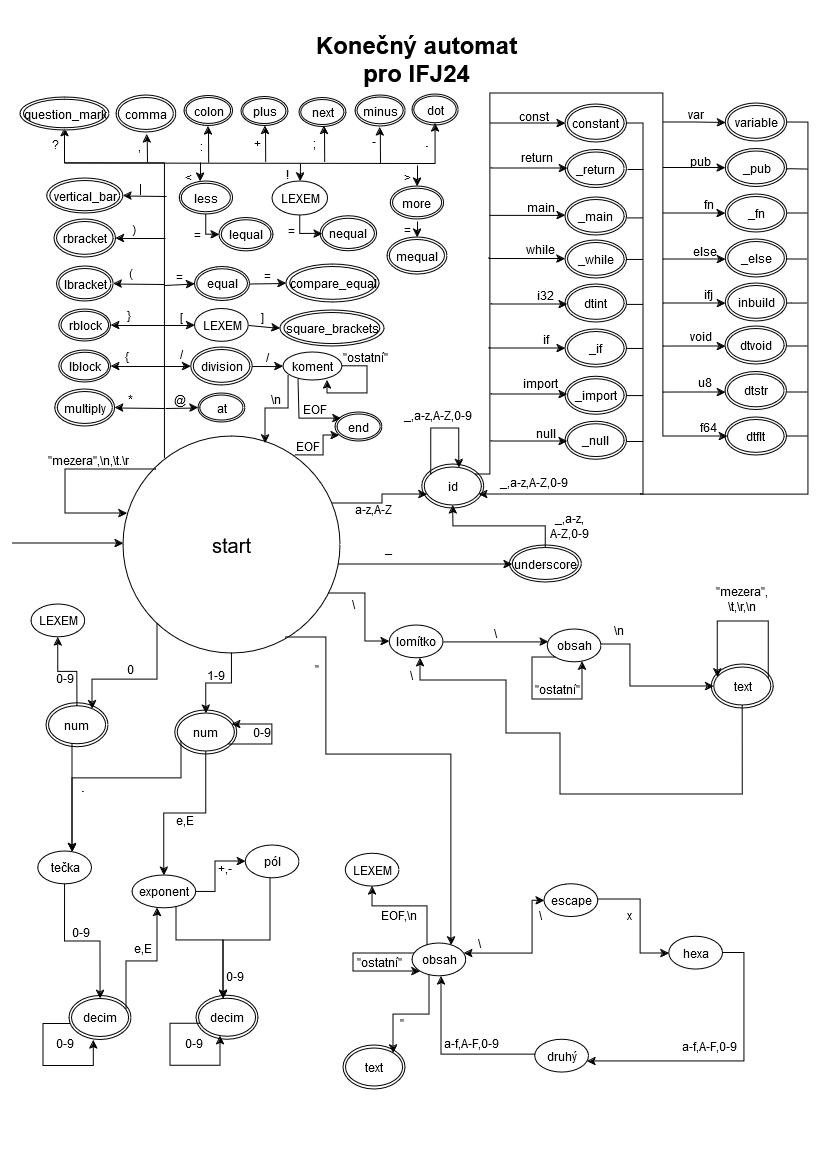
\includegraphics[origin=c, width=0.8\textwidth]{images/FSM_IFJ24.drawio.png}
        \caption{Diagram konečného automatu}
    \end{center}
\end{figure}
%%%%%%%%%%%%%%%%%%%%%%%%%%%%%%%%%%%%%%%%%%%%%%%%%%%%%%%%%%%%%%%%
\newpage
\rhead{\bfseries Implementace překladače (Syntaktická analýza)}
\subsection{Syntaktická analýza}
\subsubsection{Parser}
Syntaktická  \cite{FITPUB8538}. Načtení \textit{\textbf{next\_token()}}. uvolnění \textit{get\_next\_token()} načtení 

\subsubsection{Rozhraní mezi parserem a zpracováním výrazů (psa)}
Rozhraní \textit{\textbf{psa()}}. zapouzdřena \textit{expression()}. Jako parametr

\vspace{4cm}

\begin{figure}[ht!]
\begin{center}
\begin{tikzpicture}[square/.style={regular polygon,regular polygon sides=4}]
        \node at (0,0) [square, draw] {PARSER};
        \node at (12,0) [square, draw] {Zpracování výrazů};
        \draw (1.4,1) -- node[above]{psa()} (9.45,1);
        \draw (1.4,-1) -- node[above]{next\_token()} (9.45,-1);
\end{tikzpicture}
\caption{Rozhraní mezi parserem a zpracováním výrazů}
\end{center}
\end{figure}

\newpage

\subsubsection{LL gramatika}

\begin{enumerate}
    \item <prog> → require “ifj21” <main\_b>
    \item[]
    \item <main\_b> → function id (<params>) <ret\_func\_types> <stats> end <main\_b>
    \item <main\_b> → global id : function (<arg\_def\_types>) <ret\_def\_types> <main\_b>
    \item <main\_b> → id (<args>) <main\_b>
    \item <main\_b> → $\varepsilon$
    \item[]
    \item <stats> → local id : <type> <assign> <stats>
    \item <stats> → if exp then <stats> else <stats> end <stats>
    \item <stats> → while exp do <stats> end <stats>
    \item <stats> → return <ret\_vals> <stats>
    \item <stats> → id <id\_func> <stats>
    \item <stats> → $\varepsilon$
    \item[]
    \item <id\_func> → <n\_ids> = <as\_vals>
    \item <id\_func> → (<args>)
    \item[]
    \item <params> → id : <type> <n\_params>
    \item <params> → $\varepsilon$
    \item <n\_params> → , id : <type> <n\_params>
    \item <n\_params> → $\varepsilon$
    \item[]
    \item <n\_ids> → , id <n\_ids>
    \item <n\_ids> → $\varepsilon$
    \item[]
    \item <vals> → exp <n\_vals>
    \item <n\_vals> → , exp <n\_vals>
    \item <n\_vals> → $\varepsilon$
    \item[]
    \item <as\_vals> → <vals>
    \item <as\_vals> → id (<args>)
    \item[]
    \item <ret\_vals> → <vals>
    \item <ret\_vals> → $\varepsilon$
    \item[]
    \item <assign> → = <assign\_val>
    \item <assign> → $\varepsilon$
    \item[]
    \item <assign\_val> → exp
    \item <assign\_val> → id (<args>)
    \item[]
    \item <term> → id
    \item <term> → <const>
    \item[]
    \item <args> → <term> <n\_args>
    \item[]
    \item <args> → $\varepsilon$
    \item <n\_args> → , <term> <n\_args>
    \item <n\_args> → $\varepsilon$
    \item[]
    \item <arg\_def\_types> → <func\_def\_types>
    \item <arg\_def\_types> → $\varepsilon$
    \item[]
    \item <ret\_func\_types> → : <func\_types>
    \item <ret\_func\_types> → $\varepsilon$
    \item[]
    \item <ret\_def\_types> → : <func\_def\_types>
    \item <ret\_def\_types> → $\varepsilon$
    \item[]
    \item <func\_types> → <type>  <n\_func\_types>
    \item <n\_func\_types> → , <type>  <n\_func\_types>
    \item <n\_func\_types> → $\varepsilon$
    \item[]
    \item <func\_def\_types> → <type>  <n\_func\_def\_types>
    \item <n\_func\_def\_types> → , <type>  <n\_func\_def\_types>
    \item <n\_func\_def\_types> → $\varepsilon$
    \item[]
    \item <type> → integer
    \item <type> → number
    \item <type> → string
    \item <type> → nil
    \item[]
    \item <const> → int\_value
    \item <const> → double\_value
    \item <const> → string\_value
    \item <const> → nil
\end{enumerate}

\vspace{1cm}
Poznámka: "exp" - označení pro výraz

\newpage

\subsubsection{LL tabulka}
\begin{figure}[ht!]
\begin{center}
  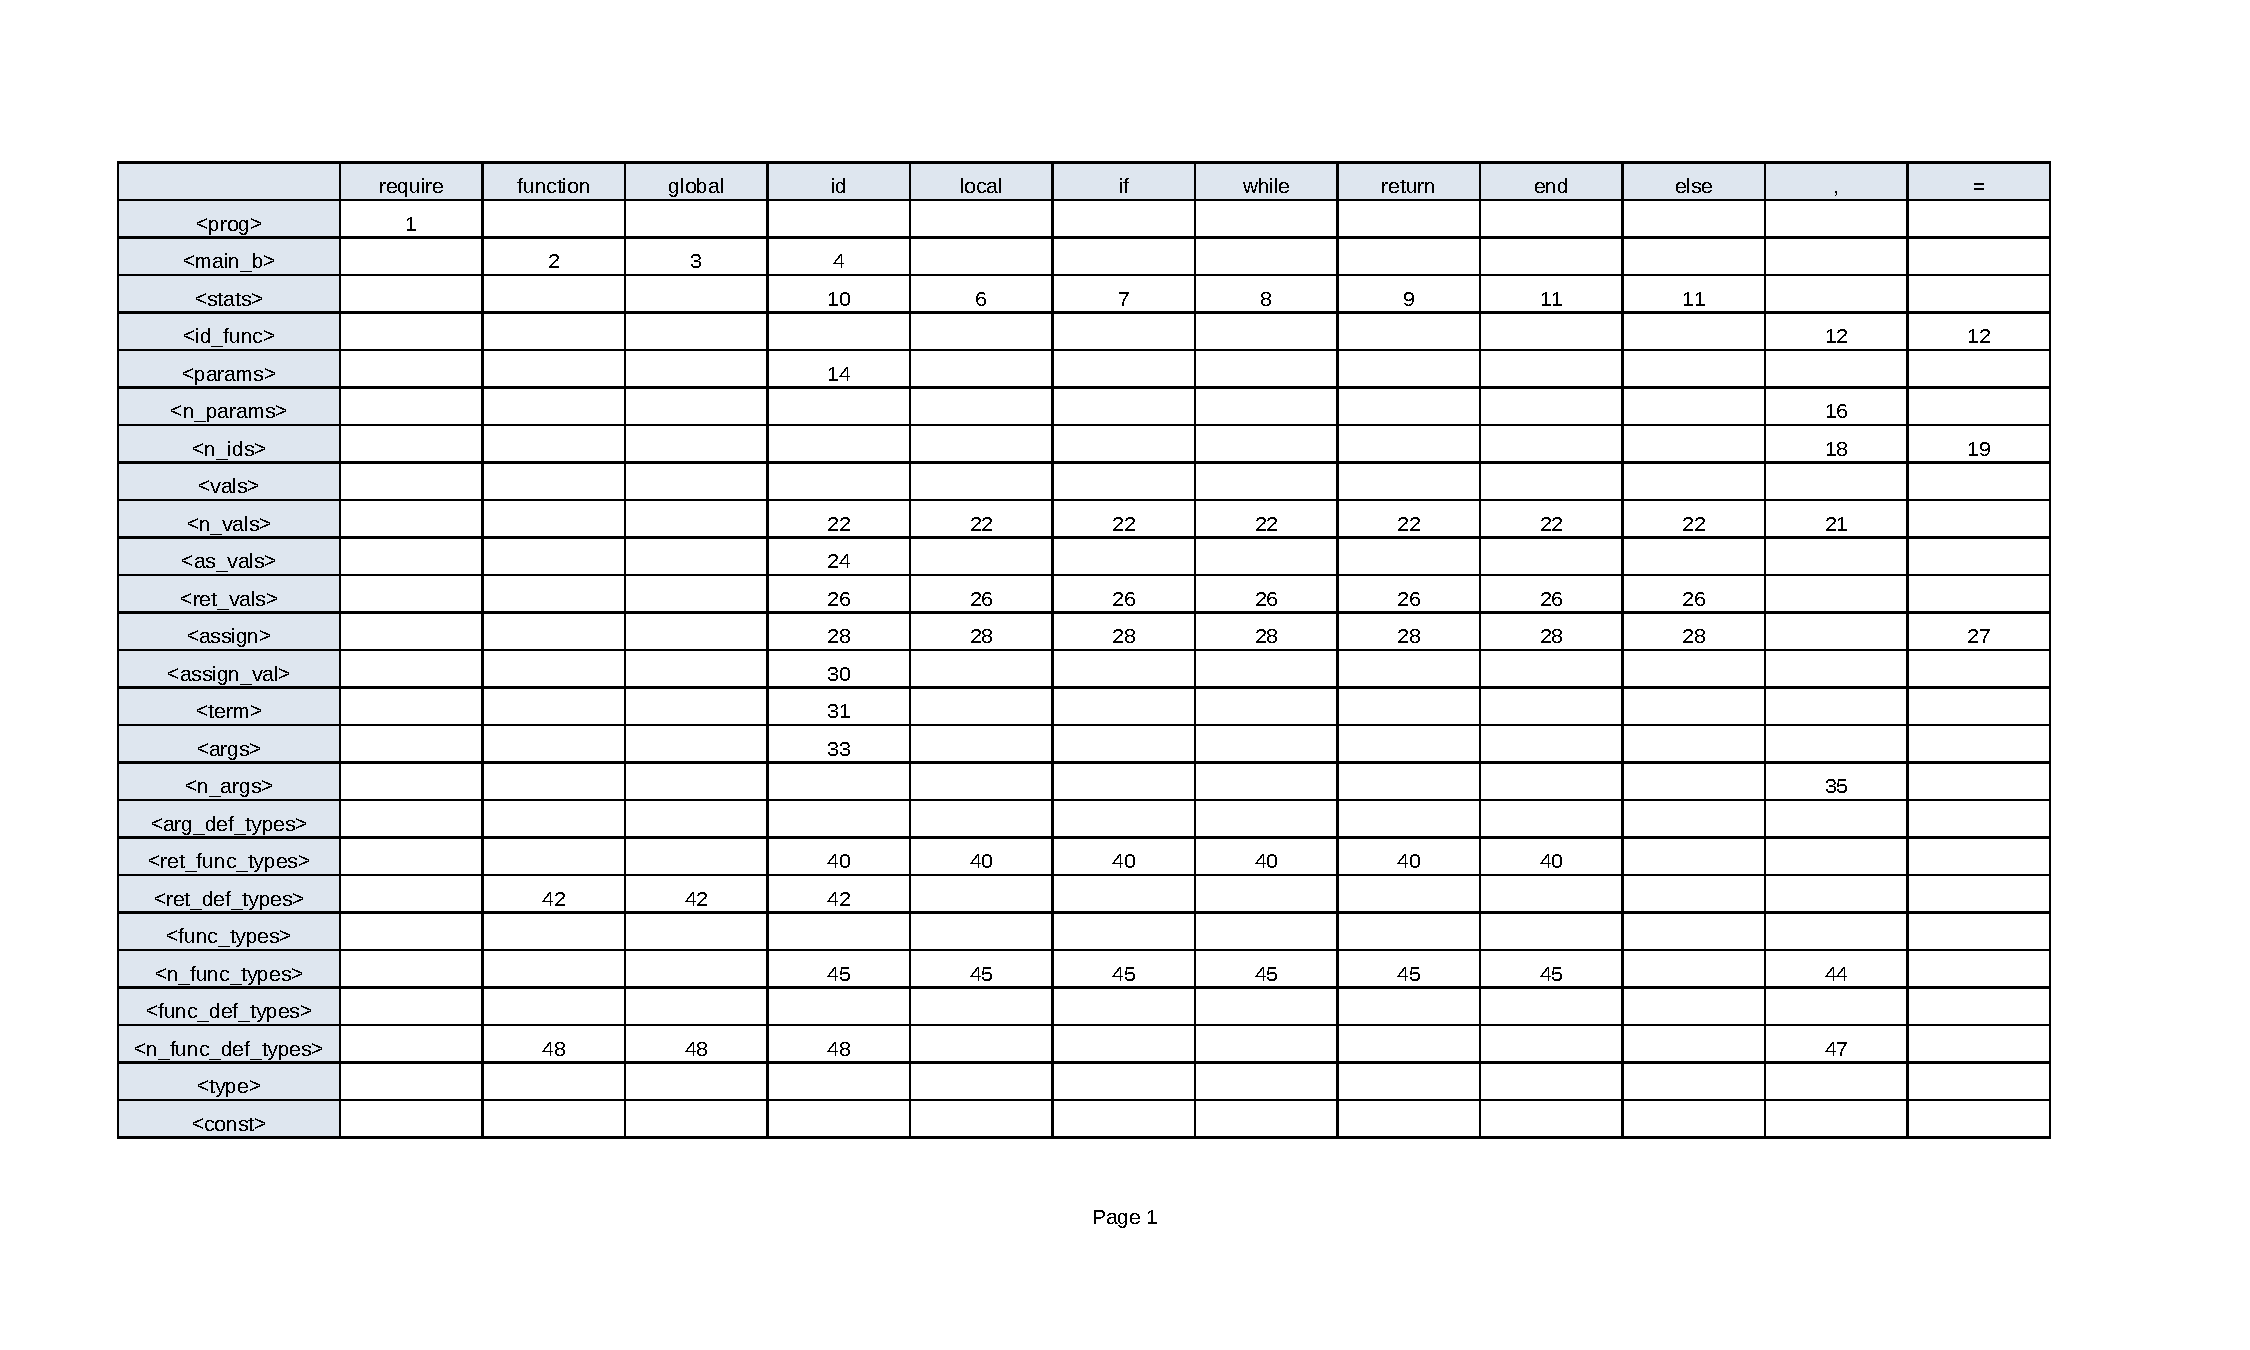
\includegraphics[angle=90,origin=c, width=0.59\textwidth, trim={0 2.5cm 0 2.5cm},clip]{images/LL_table_1.pdf}
  \caption{LL tabulka, část 1}
\end{center}
\end{figure}


\newpage

\begin{figure}[ht!]
\begin{center}
  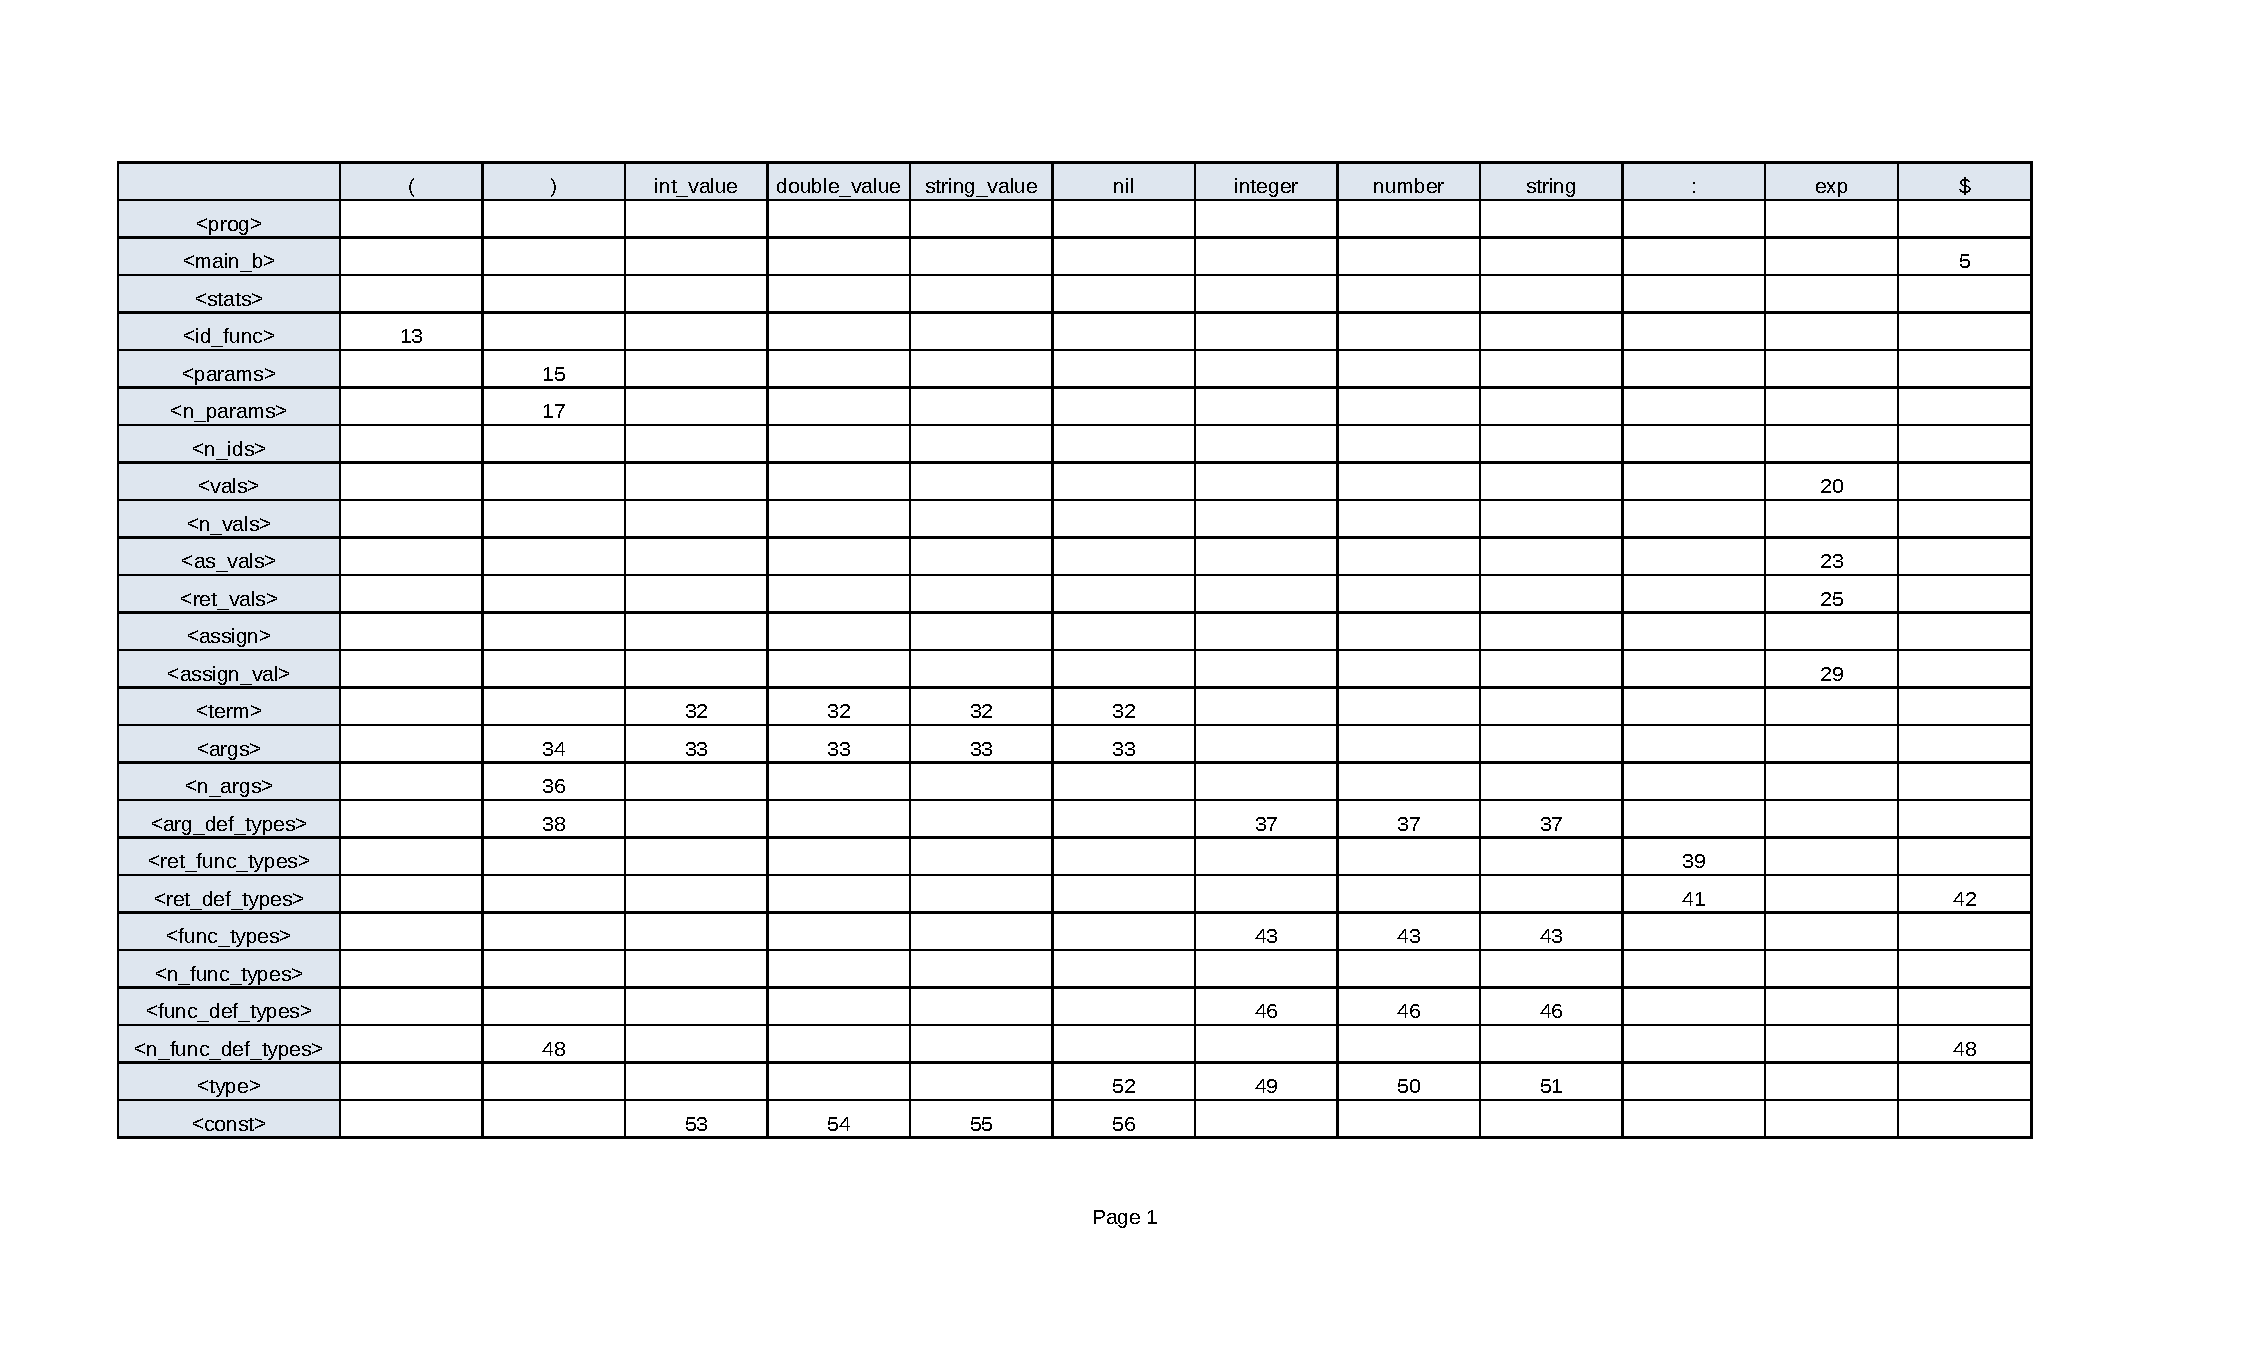
\includegraphics[angle=90,origin=c, width=0.59\textwidth, trim={0 2.5cm 0 2.5cm},clip]{images/LL_table_2.pdf}
  \caption{LL tabulka, část 2}
\end{center}
\end{figure}

\newpage

\subsubsection{Zpracování výrazů}
Zpracování \textit{psa.c (.h)} prováděno \cite{FITPUB8538}. Nejprve \textit{psa\_table\_symbol\_enum} načten \textit{\textbf{get\_index\_enum()}} funkce

\subsubsection{Precedenční tabulka}
\begin{figure}[ht!]
\begin{center}
  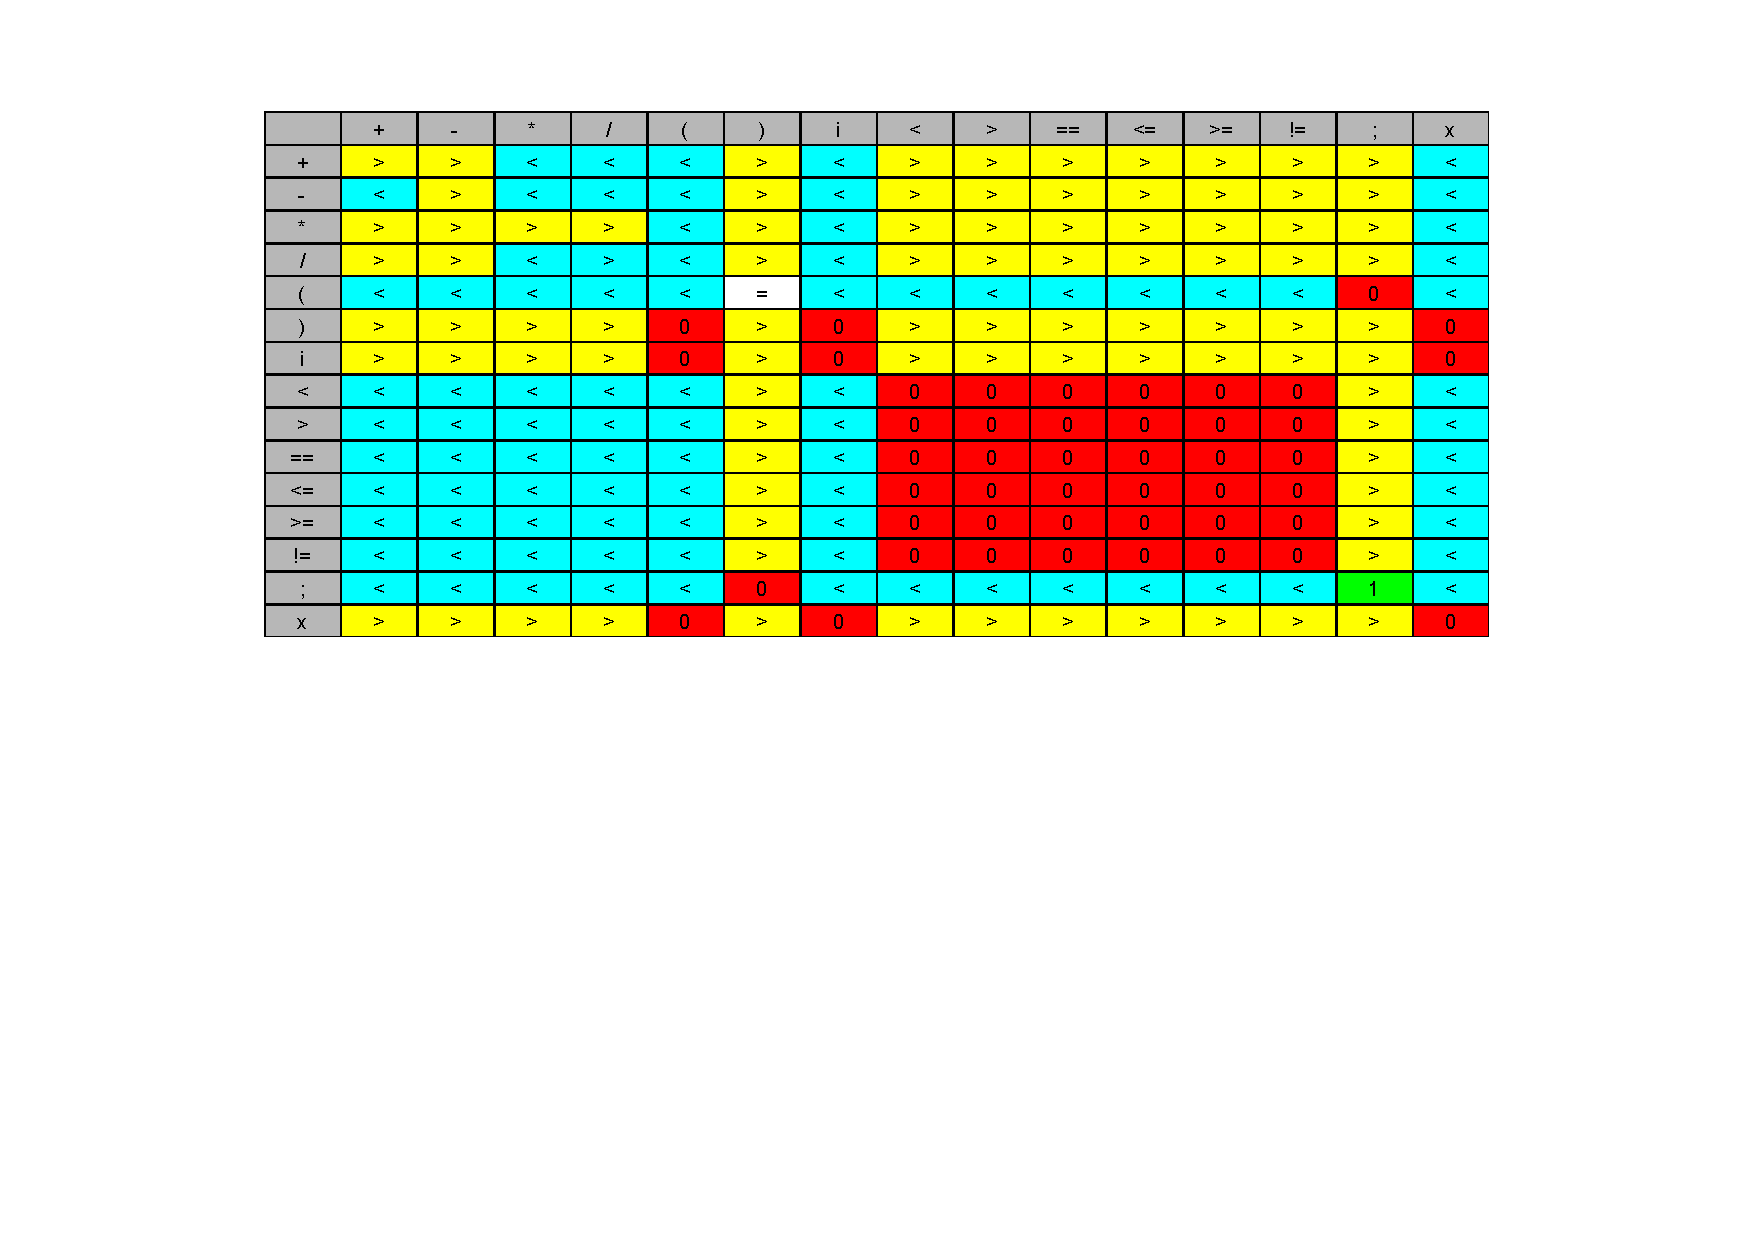
\includegraphics[width=1\textwidth, trim={0 2.5cm 0 0},clip]{images/precedence_table.pdf}
  \caption{Precedenční tabulka}
\end{center}
\end{figure}

\newpage

\subsubsection{Gramatika pro výrazy}

\begin{enumerate}
    \item E → i
    \item E → $\#$E
    \item E → (E)
    \item E → E $..$ E
    \item E → E $+$ E
    \item E → E $-$ E
    \item E → E $*$ E
    \item E → E $/$ E
    \item E → E $//$ E
    \item E → E $=$ E
    \item E → E $\sim=$ E
    \item E → E $<=$ E
    \item E → E $>=$ E
    \item E → E $<$ E
    \item E → E $>$ E
\end{enumerate}

%%%%%%%%%%%%%%%%%%%%%%%%%%%%%%%%%%%%%%%%%%%%%%%%%%%%%%%%%%%%%%%%%%%%%
\newpage
\rhead{\bfseries Implementace překladače (Tabulka symbolů)}
\subsection{Tabulka symbolů}
Dle výběru varianty zadání \rom{1} je tabulka symbolů implementována binárním vyhledávacím stromem. Ten je implementován v souboru \textit{symtable.c (.h)}.

\subsubsection{Návrh tabulky symbolů}
Prvek v tabulce symbolů obsahuje následující elementy:

\vspace{1cm}

\begin{itemize}
    \begin{minipage}{0.3\linewidth}   
    \item declared
    \item defined
    \item data\_type
    \item params\_count
    \item params\_type\_count
    \item returns\_def\_count
    \item returns\_count    
    \item first\_param
    \item first\_type\_param
    \item first\_def\_ret
    \item first\_ret
    \end{minipage}
    \begin{minipage}{0.65\linewidth}   
    \item[-] proměnná/funkce byla deklarována
    \item[-] proměnná/funkce byla definována
    \item[-] datový typ proměnné
    \item[-] počet parametrů definice funkce
    \item[-] počet parametrů deklarace funkce
    \item[-] počet návratových typů definice funkce
    \item[-] počet návratových typů deklarace funkce    
    \item[-] ukazatel na první parametr definice funkce
    \item[-] ukazatel na první parametr deklarace funkce
    \item[-] ukazatel na první návratový typ definice funkce
    \item[-] ukazatel na první návratový typ deklarace funkce
    \end{minipage}
\end{itemize}

\vspace{1cm}

Všechny \textit{symData\_t}. Při inicializaci

Jako element

\newpage

\subsubsection{Uložení tabulek symbolů do jednosměrně vázaného seznamu}
Jednotlivé \textit{sym\_linked\_list.c (.h)}. Tento

\vspace{4cm}

\begin{figure}[ht!]
\begin{center}
\begin{tikzpicture}[list/.style={rectangle split, rectangle split parts=2,
    draw, rectangle split horizontal}, >=stealth, start chain]

  \node[list,on chain] (A) {lok. tab. symb. *};
  \node[list,on chain] (B) {lok. tab. symb. *};
  \node[list,on chain] (C) {glob. tab. symb. *};
  \node[on chain,draw,inner sep=6pt] (D) {};
  \draw (D.north east) -- (D.south west);
  \draw (D.north west) -- (D.south east);
  \draw[*->] let \p1 = (A.two), \p2 = (A.center) in (\x1,\y2) -- (B);
  \draw[*->] let \p1 = (B.two), \p2 = (B.center) in (\x1,\y2) -- (C);
  \draw[*->] let \p1 = (C.two), \p2 = (C.center) in (\x1,\y2) -- (D);
\end{tikzpicture}

\tikzset{every tree node/.style={minimum width=2em,draw,circle},
         blank/.style={draw=none},
         edge from parent/.style=
         {draw,edge from parent path={(\tikzparentnode) -- (\tikzchildnode)}},
         level distance=1.5cm}
\begin{tikzpicture}[sibling distance=25pt]
\Tree
[.ida     
    [.idb ]
    [.idc 
    \edge[blank]; \node[blank]{};
    \edge[]; [.idd
         ]
    ]
]
\end{tikzpicture}
\begin{tikzpicture}[sibling distance=25pt]
\Tree
[.ide     
    [.idf ]
    [.idg 
    \edge[blank]; \node[blank]{};
    \edge[]; [.idh
         ]
    ]
]
\end{tikzpicture}
\begin{tikzpicture}[sibling distance=30pt]
\Tree
[.i()      
    [.j()  ]
    [.k()  
    \edge[blank]; \node[blank]{};
    \edge[]; [.l()
         ]
    ]
]
\end{tikzpicture}
\vspace{2cm}

* - ukazatel na kořen binárního stromu reprezentujícího tabulku symbolů \newline

\caption{Diagram jednosměrně vázaného seznamu}
\end{center}
\end{figure}

%%%%%%%%%%%%%%%%%%%%%%%%%%%%%%%%%%%%%%%%%%%%%%%%%%%%%%%%%%%%%%%%%%%%%%%%%%%%%%%
\newpage
\rhead{\bfseries Implementace překladače (Sémantická analýza)}
\subsection{Sémantická analýza}
\subsubsection{Parser}
Sémantický \textit{parser.c} Zmíněný

\subsubsection{Zpracování výrazů}
Psa provádí \textit{\textbf{get\_type()}} Při redukci 

\subsection{Generování kódu}
\subsubsection{Vlastní generování kódu}
případů \textit{scale} přidávána

\subsubsection{Rozhraní generátoru kódu}
rozhraní \textit{codeGen\_ ... ()} a ve tvaru \textit{generate\_ ... ()}. Každá v souboru \textit{code\_generator.c (.h)}.

\vspace{0.75cm}

\begin{figure}[ht!]
\begin{center}
\begin{tikzpicture}[square/.style={regular polygon,regular polygon sides=4}]
        \node at (0,0) [square, draw] {PARSER, PSA};
        \node at (12,0) [square, draw] {Generátor kódu};
        \draw [line width=0.75mm] (2.15,0) -- node[above]{codeGen\_ ... (), generate \_ ... ()} (9.8,0);
\end{tikzpicture}
\caption{Rozhraní mezi parserem, psa a generátorem kódu}
\end{center}
\end{figure}

%%%%%%%%%%%%%%%%%%%%%%%%%%%%%%%%%%%%%%%%%%%%%%%%%%%%%%%%%%%%%%%%%%%%%%%%%%%%%%%%%%%%%
\newpage
\rhead{\bfseries Datové struktury a datové typy}
\section{Datové struktury a datové typy}
\subsection{Datové struktury}

\subsubsection{Zásobník symbolů (zpracování výrazů)}
Zásobník \textit{symstack.c (.h)}. Zmíněný \textit{\textbf{symbol\_stack\_insert\_after\_top\_terminal()}}. Funkce

\subsubsection{Zásobník parametrů (parser)}
Zásobník \textit{paramstack.c (.h)}

\subsubsection{Binární vyhledávací strom (tabulka symbolů)}
Binární \textit{symtable.c (.h)}. Jeho \cite{pruvodce2017}. Při 

\subsubsection{Jednosměrně vázaný seznam (tabulka symbolů)}
Jednosměrně \textit{sym\_linked\_list.c (.h)}. Jako

\subsubsection{Jednosměrně vázaný seznam (identifikátory)}
Jednosměrně \textit{ids\_list.c (.h)}. Jeho 

\subsubsection{Obousměrně vázaný seznam (generování kódu)}
Obousměrně \textit{dll.c (.h)}. Slouží \textit{\textbf{DLL\_InsertLast()}}, pomocí \textit{\textbf{DLL\_PrintAll()}}

\subsection{Datové typy}
\subsubsection{string\_t}
Datový \textit{string\_t} implementován

\subsubsection{token\_t}
Datový \textit{token\_t} implementován

\newpage

\rhead{\bfseries Reference}
\bibliographystyle{plain}
\bibliography{reference.bib}

\end{document}
